\documentclass{article}
\usepackage{tikz}
\usetikzlibrary{shapes,shadows,arrows}
\usepackage{pgfplots,pgfplotstable}

\usepackage{fp}

\begin{document}

\begin{figure}[ht]
	\centering
	\begin{center}
		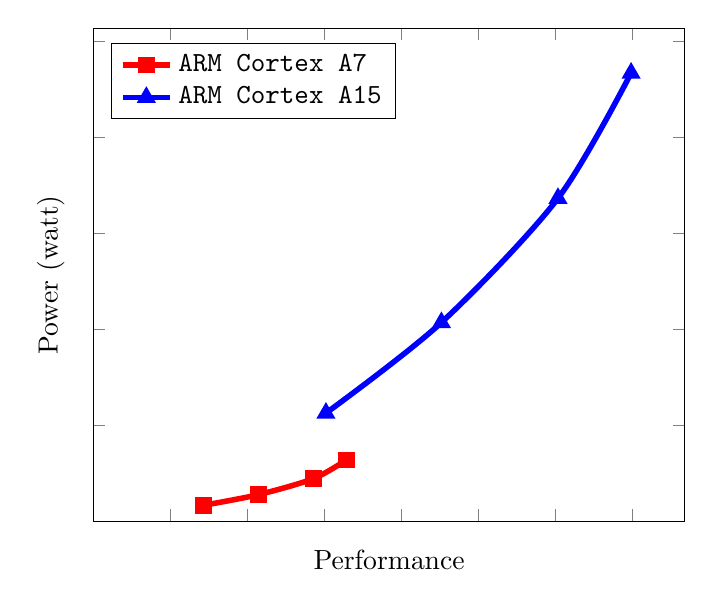
\begin{tikzpicture} %[>=latex]
		\begin{axis}[
		width=0.75\textwidth,
		%line width=2,
		%symbolic x coords={2012, 2013, 2014, 2015, 2016},
		xticklabels={,,},
		yticklabels={,,}
		%xticklabels={720p,1080p,4k},
		%minor xtick={0,1,...,18},
		grid=both,
		ymin=0,
		xmin=0,
		xlabel=Performance,
		ylabel=Power (watt),
		legend pos=north west,
		legend cell align=left,
		%enlarge x limits=0.1,
		%xticklabel style={text width=0.2\textwidth,align=flush left},
		]
		\addplot[line width=2pt,smooth,color=red,mark=square*] coordinates {
			(20/28,3/18)
			(30/28,5/18)
			(40/28,8/18)
			(46/28,11.5/18)
		};
		\addplot[line width=2pt,smooth,color=blue,mark=triangle*] coordinates {
			(42.3/28,20.3/18)
			(63.3/28,37.3/18)
			(84.5/28,60.6/18)
			(97.8/28,84.1/18)
		};
		\legend{\texttt{ARM Cortex A7~}\\\texttt{ARM Cortex A15}\\}
		%\draw[red] plot [smooth] coordinates {(0 0) (2,3700) (4,6006) (18,18000)};
		\end{axis}
		\end{tikzpicture}
	\end{center}
	\caption{Bandwidth required for delivering various videos.}\label{fig:bitrate-resolution}
\end{figure}

\end{document}